
 \chapter{Background}\label{ch:background}
Every year 37.3 million falls occur that are severe enough to require medical attention [1]. Elderly people, in particular, tend to suffer the largest number of fatal falls. [7] Each year, one in four people over the age of 60 experience a fall, and one in three people over the age of 65 experience a fall. Falls remain one of the leading reasons for elderly admissions to the hospital at a rate of 38\%, and the second-largest cause being vehicle injuries at a rate of 13\%.

The health direct [6] states that a fall usually occurs due to gradual changes in our bodies that make walking difficult or hazards inside the current environments. The changes that occur due to aging tend to be balance issues, weakening muscles that make it harder to walk, degradation in eyesight, and slower reaction times. 

Falls have a severe risk involved, the most common injuries being fractures to the thigh and hip at 38\%, followed by injuries to the head at 20\%. Falls cause more injury deaths in Australia than car collisions. To help visualise the impact of falls, A Western Australian dies every 26 hours, is admitted to a hospital every 19 minutes, and presents to an emergency room every 12 minutes due to falls. According to the CDC [9], amongst people over the age of 65, \$50 billion is spent on medical costs related to non-fatal fall injuries, and \$754 million is spent related to fatal falls. These costs cover hospital feels, doctor checkups, rehabilitation, medical equipment, prescripted drugs, and insurance.

These issues have led to the requirement for fall detection technology to acquire immediate response. If an individual has fallen over and is rendered unconscious, they are at significant risk and are unable in any way to seek help. In the modern-day and age, fall detection is performed through a variety of different techniques, illustrated in Table 2.1.\\


\begin{table}[htp]
    \centering
    \begin{tabular}{ |p{3.5cm}|p{3.0cm}|p{2.5cm}|p{2.6cm}|}
     \hline
     \multicolumn{4}{|c|}{Fall Detection Method} \\
     \hline
     Technique& Type &Machine Learning Type&category\\
     \hline
     \hline
     push-button alarm system&wearable sensor&N/A&non-automated\\
     \hline
     mobile phone/smartwatch&wearable sensor&N/A&automated\\
     \hline
     wearable pendants&wearable sensor&supervised learning&automated\\
     \hline
     camera based monitoring&ambient sensor&supervised learning&automated\\
     \hline
     IR monitoring&ambient sensor&semi-supervised learning&automated\\
     \hline
     mmWave monitoring&ambient sensor&semi-supervised learning&automated\\
     \hline
    \end{tabular}
    \caption{Fall detection techniques established in current date.}
\end{table}

It is also worth noting that fusing information from different types of sensors for fall detection has been a new area of research. In a study performed by \textit{G. Koshmak et al.} [27] multiple types of sensors were fused to determine the effect on accuracy. When combining wearable sensors, accuracy had increased; however, numerous digital devices had to be attached to an individual's body, requiring even more responsibility and inconveniencing the individual. 

This study had also investigated fusing wearable sensors and ambient sensors. In most cases, the fusion had increased accuracy compared to each sensor component. However, this approach is still new and actively being researched. Each fusion requires a unique algorithm and testing. 

Research in the field of fall detection can be categorised into two major categories, automated and non-automated. The following section will outline the groundwork for both methods.

\section{Non-Automated Fall Detection}
\subsection{Push-Button Alarm Systems}
Push-button alarm systems work by sending an alarm when an individual presses the button on their supplied wearable technology. Typical push-button alarms are displayed below in Figure 2.1.\\

\begin{figure}[htp]
    \centering
    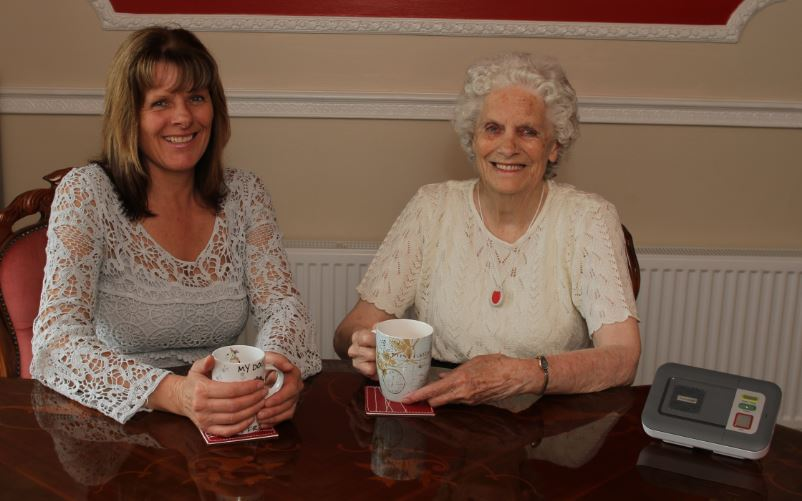
\includegraphics[width=400px,height=400px,keepaspectratio]{wearable-sensor.jpg}
    \vspace{-2ex}%
    \caption{A typical wearable push-button alarm worn around the neck. (SureSafe, 2021)}
    \label{fig:my_label}
\end{figure}

Upon falling, the individual would press the button located on the device to signal for an alert. The individual is free to chose the location of the device, as they bear personal responsibility for the usage of the device.

However, these methods have been shown in studies from \textit{Fleming et al.} [10] to be often ineffective at dealing with more dangerous falls. In the year of investigation on 265 fall reports, 82\% of falls occurred when the individual was isolated. Of the 60\% of people who had fallen, 80\% of them were unable to get up afterward, and 30\% had laid on the floor for over an hour. A large portion of the study population was using push-button alarms; however, barriers of use arose. If an individual is unconscious after falling, they are unable to activate their alarm. There was also the issue of many individuals who had a device available but were not wearing it during their falls. Often this was due to forgetfulness or the individuals decision to not wear their alarms.

\section{Automated Fall Detection}
Automated fall detection attempts to take the responsibility off the user by automating the process of sending the alarm. This approach can be broken down into two different categories, dataless methods and data-driven methods.
\subsection{Dataless Methods}
Dataless fall detection methods are a branch of fall detection that only requires current motion information to detect falls. Typically wearable sensors are used for dataless methods, and often this approach is seen as the evolution of push-button alarm systems. The sensors work in a similair regard to being worn by the individual; however, algorithms in place can automatically detect falls and alert an emergency contact or carer. Typically these systems are in place on smartphones, smartwatches and pendants. [11] These systems work through motion detection by using an accelerometer and a gyroscope located inside the devices. These sensors are designed to detect everyday activity and the motion of a fall. The accelerometer measures the change in velocity divided by time; this is the technology that changes screen view on a phone when rotated. The gyroscope is a device used to determine the orientation using the earth's gravity, allowing the tracking of rotational information. Custom algorithms are in place to accurately sense when falls take place. Figure 2.2 shows the general flow of this fall detection methodology. 

\begin{figure}[H]
    \centering
    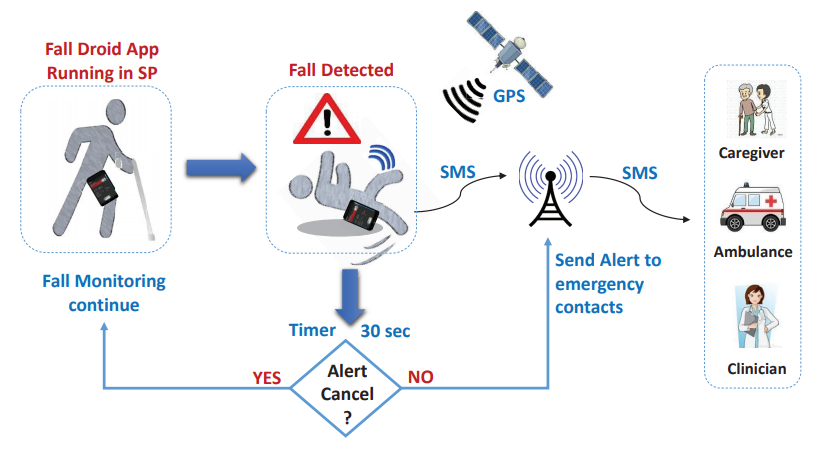
\includegraphics[width=400px,height=400px,keepaspectratio]{fall detection flow.png}
    \vspace{-2ex}%
    \caption{Fall detection flow for wearable technology. (Shahzad, 2018)}
    \label{fig:my_label}
\end{figure}

These fall detection methods are a significant improvement to a push-button alarm system as they take most of the responsibility away from the user. However, they still require the user to always have the devices on them and making sure their device is charged. In particular, the pendants need the user to be in proximity to the connector that sends the alert. 

\subsection{Data-driven Methods}
Data-driven fall detection is a method of fall detection that uses previous fall data information to predict whether a fall has occurred or not. Typically machine learning or deep learning is used for these approaches. Machine learning is learning through examples and classifying new samples based on weights learned during training. Deep learning is an extension of machine learning that uses multi-layered neural networks to perform more powerful classification. We can often categorise machine learning and deep learning into three major sections, supervised learning, unsupervised learning, and semi-supervised learning. 

The following section will outline the difference between the different categories of machine learning and deep learning. All sections discussed that are not directly classified as machine learning can be assumed to be deep learning.


\subsubsection{Supervised Learning}
Supervised learning is a branch of machine learning that learns how to fit incoming example data to a specific class output. This can also be seen as predicting an output class based on the incoming data. A straightforward example would be a model that indicates whether a person earns a salary over \$50,000 based on the person's occupation, age, and other characteristics. However, this process requires labelled data to train up a model. Labelled data is where each feature is defined for the example data input. Figure 2.3 displays an outline of data used in supervised learning. As shown, a combination of gender, age, and salary is used to predict the output class purchased (whether or not the person has purchased the item).

\begin{figure}[H]
    \centering
    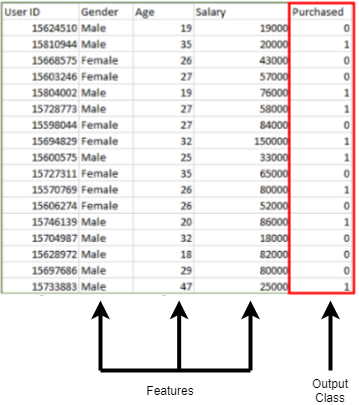
\includegraphics[width=200px,height=250px]{MLdata.png}
    \vspace{1ex}%
    \caption{Labelled data for a simple supervised learning classifier. (GeeksForGeeks, 2020)}
    \label{fig:my_label}
\end{figure}

For fall detection, typically, the input would be a video stream passed into a model. Each frame of the video's pixel data is split into three colour channels for RGB, and other times the data would be motion information. The following section will explain the types of models used for supervised learning for fall detection.

\paragraph{Machine Learning Approaches}\mbox{}\\\\
Fall detection using traditional machine learning is typically used with wearable sensors. The model on the wearable device attempts to learn the motion of a fall using accelerometers and gyroscopes (similair to section 2.2.1); however, rather than using inbuilt algorithms to do a simple fall check, motion data is used as input for a trained model to detect falls. 

In an article written by \textit{Palmerini et al.} [18], sensors worn on the lower back would track motion data with an accelerometer. One hundred and forty-three simulated falls were gathered from 40 subjects within the group's age range, 69.2 $\pm$ 12.7. In addition to fall data, regular activities of daily living (ADL) data was also recorded from 15 subjects to offer a comparison, none of which had performed a fall. 

Many models were used to observe the performance and provide comparisons; this included Naïve Bayes, logistic regression, K-Nearest Neighbour (KNN), random forests, and Support Vector Machines (SVM). Motion data was passed into each model, and one-class classification is performed to output whether a fall occurred or not. 

The results of this study showed extremely high specificity with these techniques. Table 2.2 outlines the stand-out traditional machine learning techniques and their specificity for this study. 

\begin{table}[H]
    \centering
    \begin{tabular}{ |p{3.5cm}|p{3cm}|p{4.3cm}|}
     \hline
     \multicolumn{3}{|c|}{Results of classification} \\
     \hline
     Model &Specificity & False Alarm Rate hourly\\
     \hline
     Naïve Bayes&99.1\%&1.09\\
     Logistic Regression&99.3\%&0.76\\
     KNN&99.2\%&0.92\\
     SVM&99.5\%&0.56\\
     Random Forests&98.9\%&1.32\\
     \hline
    \end{tabular}
    \caption{Result of classification from traditional machine learning approach. (Palmerini, 2020)}
\end{table}

While these models have very high specificity, this was likely due to the models being heavily biased towards detecting falls. This can be seen from the false alarm rates, which are incredibly high. Due to the high rate of false alarms, this system would be unviable as a means of fall detection.
\paragraph{Convolutional Neural Networks}\mbox{}\\

In the case of fall detection using convolutional neural networks (CNN), many approaches can be taken. The first approach is to take the optical flow of an image to capture motion history and using a 3D CNN combined with transfer learning. Another method would be to use a 3D CNN and stacking multiple frames together as input. Finally, another approach is to use mmWave data in a deep 2D CNN. 

In a study performed by \textit{Ji et al.} [14], 3D CNN's were used to detect human activities on TRECVID data which consists of 49 hours of video footage from London airport. The study had focused on recognising three different human actions, putting a cellphone to the ear, pointing, and placing an object somewhere. Alongside having data on these cases, many negative samples were inserted where none of these actions were present in the samples. The model used for this study is shown below in Figure 2.4. 

\begin{figure}[H]
    \centering
    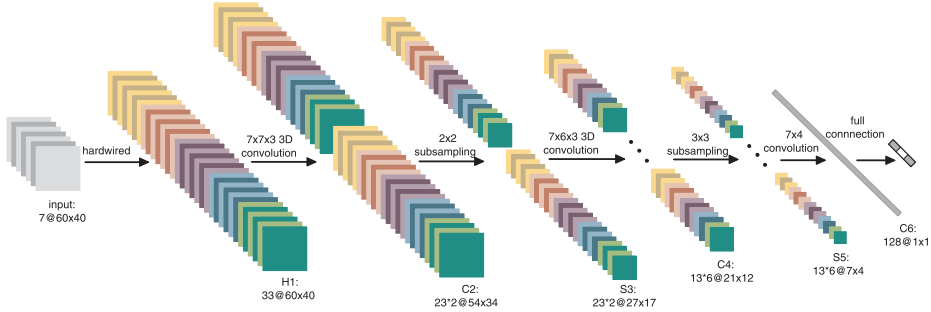
\includegraphics[width=400px, keepaspectratio]{conv1.png}
    \vspace{1ex}%
    \caption{CNN structure for the study on human activity recognition. (Ji, 2013)}
    \label{fig:my_label}
\end{figure}

While this study did not directly detect falls, the extension is that human activity recognition can be extended to also include falls amongst the activities listed and potentially even more. The results from this study had shown that under a false positive rate of 0.1\%, the model had on average 71.48\% precision, 2.43\% recall, and an AUC value of 0.0139. Using a false positive rate of 1\%, the model had an average  55.84\% precision, 11.47\% recall, and an AUC value of 0.6993. This approach had outperformed all other state-of-the-art models such as  2D CNNs and spatial pyramid matching SVMs. However, it is worth mentioning that the CellToEar precision and recall were typically much lower than ObjectPut and Pointing for the results. This could be due to the action of bringing a cellphone to the ear being much more complex than simply putting down an object or pointing at something. It is also worth mentioning that having as high specificity as possible for fall detection is the main priority. Misclassifying a fall as a false negative could be the difference between life and death. This model's low accuracy would be unsuitable for fall detection, especially when other models have been shown to perform with much higher accuracy. 

In another study performed by \textit{Núñez-Marcos et al.} [15], 3D CNN's were used to detect falls on simulated fall data through the use of transfer learning. This study had first converted each video frame into an optical flow image. The horizontal and vertical vector fields were separated and passed into the CNN as a stack similair to the previous study. The model used for this study is displayed below in Figure 2.5 and is very deep with many convolving layers. Finally, three fully connected layers are then softmaxed to predict the binary classification if the example was a fall or not.

\begin{figure}[H]
    \centering
    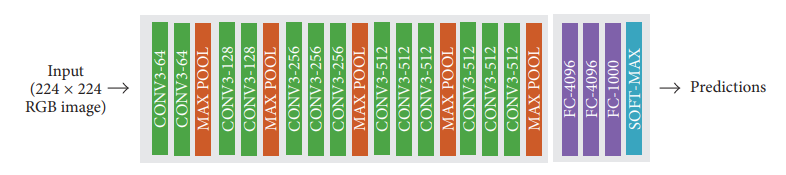
\includegraphics[width=400px, keepaspectratio]{othercnn.png}
    \vspace{1ex}%
    \caption{CNN structure for the study on fall detection using optical flow. Keep note the input is the stacked horizontal and vertical optical flow images. (Núñez-Marcos, 2017)}
    \label{fig:my_label}
\end{figure}


Transfer learning was used to account for the lack of public fall data. First, the CNN was trained on the Imagenet images dataset. Next, the model was trained on the UCF101 action recognition dataset, using optical flow images for input. Finally, the CNN was frozen during training (no weight updates) to fine-tune the final fully connected layers. A sequence of frames was extracted using a sliding window approach to extract the frames where fall or no fall sequences occur.

A sliding window approach was used to bunch incoming sequences of frames to preserve the motion history within the series of frames. The specific approach taken was to use a step of one which makes sure that no motion history is lost. However, this causes training and classification to be slower. Figure 2.6 displays a visual representation of the sliding window approach. It would be interesting to research further the performance vs. efficiency trade-off between different step sizes for a sliding window approach.

\begin{figure}[H]
    \centering
    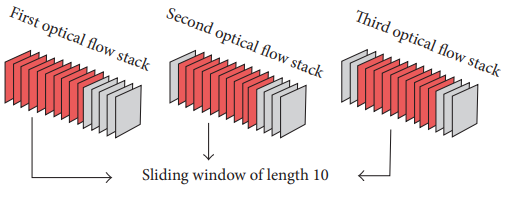
\includegraphics[width=400px, keepaspectratio]{aaaaa.png}
    \vspace{1ex}%
    \caption{Sliding window approach used to maintain motion history. (Núñez-Marcos, 2017)}
    \label{fig:my_label}
\end{figure}

This study showed that it was challenging to learn how to classify the "fall" class. In particular, attempts were made to improve the importance of the fall class, such as adding bias to the fall class in the learning. While this proved to increase the classification of falls significantly, it did come at the cost of more false positives. Three different fall datasets were used for testing, UR fall dataset (URFD), fall detection dataset (FDD), and multiple cameras fall dataset (Multicam). The model had shown extremely high sensitivity, which is how good the system predicts falls, and the model has shown high specificity. On the URFD dataset, the model had a 100\% sensitivity rate and 94.86\% specificity rate. On the FDD dataset, the model had a 93.47\% sensitivity rate and 97.23\% specificity rate. On the Multicam dataset, the model had a 98.07\% sensitivity rate and 96.20\%. This method produces exceptionally high accuracy and would be a suitable fall detection model. However, it does come with the issue of privacy concerns. Figure 2.7 shows the data involved with this classification type, which flags privacy concerns as this data is stored by a third party, constantly monitoring individuals. 

\begin{figure}[H]
    \centering
    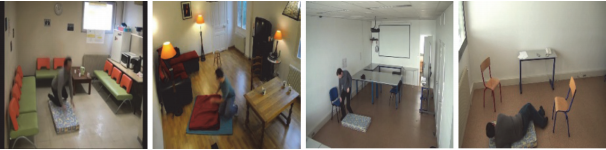
\includegraphics[width=400px, keepaspectratio]{falllll.png}
    \vspace{1ex}%
    \caption{Camera feed footage for the proposed CNN model. (Núñez-Marcos, 2017)}
    \label{fig:my_label}
\end{figure}

\textit{Jin et al.} [15] performed a study to detect patient activity, primarily fall detection using millimeter wave (mmWave) Radar and Deep CNNs. This developed model was able to distinguish patients and perform activity recognition on all the patients. The model would first detect the multiple patients from the radar using custom-built algorithms. Doppler features for each patient were then passed into a deep CNN. This model is shown below in Figure 2.8

\begin{figure}[H]
    \centering
    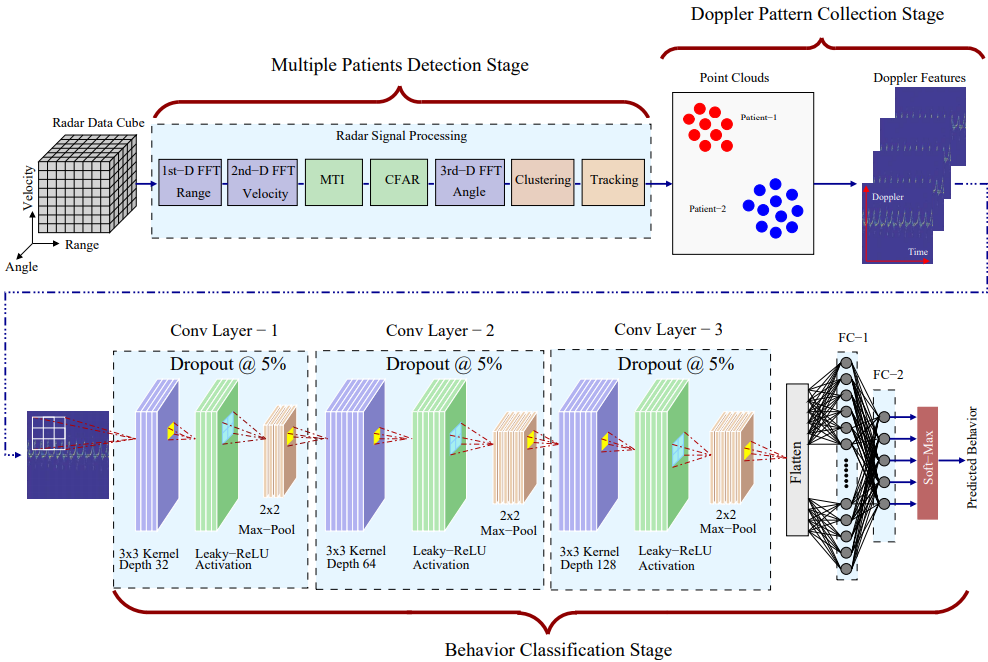
\includegraphics[width=400px, height=270px]{conveee.png}
    \vspace{1ex}%
    \caption{CNN structure and data extraction used for proposed model. (Jin, 2019)}
    \label{fig:my_label}
\end{figure}

The model in this study was able to classify behaviour into the following categories: walking, falling, swinging hand for help, seizure, and restless movement. The data used for this study was simulated falls with only one patient. 

\begin{comment}Table 2.2 shows the training dataset used in this study.  
\begin{table}[htp]
    \centering
    \begin{tabular}{ |p{4.5cm}|p{3cm}|p{3cm}|}
     \hline
     \multicolumn{3}{|c|}{Training Dataset} \\
     \hline
     Action&Samples &Label\\
     \hline
     Other&41,788&0\\
     Walking&11,201&1\\
     Falling&5,745&2\\
     Swing&10,719&3\\
     Seizure&10,299&4\\
     Restless Movement&17,216&5\\
     \hline
    \end{tabular}
    \caption{Distribution of samples used in training for proposed model in study.(F. Jin, 2019)}
\end{table}
\end{comment}
One issue that arose with this fall detection method was defining a robust dataset that covers all kinds of situations, as when a fall was in another direction, the fall was misclassified.  

The result of this study was based on the number of patients in the frame. When performing behaviour prediction on one patient, specifically for falling, the inference accuracy was 84.49\%, adding another user to the frame had significantly decreased the inference accuracy to 66.02\%. This is likely due to the increased complexity of the task to classify multiple people separately, and possibly deepening the network or training for more epochs may be needed to improve this accuracy. 

A major advantage of this approach was the ability to maintain the privacy of individuals due to the data used for classification. Video footage is not taken from subjects, and subjects are displayed as many points, illustrated in the data collection portion of Figure 2.8.

\subsubsection{Unsupervised Learning}
Unsupervised learning is a branch of machine learning that attempts to discover patterns and information in data to create clusters and grouping. This approach has major benefits for anomaly detection. Typically autoencoders make excellent models for unsupervised anomaly detection.

In a study conducted by \textit{Kiran et al.} [29], many deep networks were used to determine anomalies in video data. UCSD and CUHK-Avenue datasets were used to evaluate the performance of all models and allow comparison. Both the optical flow and raw image sequences were used as input.

This study showed that deeper autoencoder models struggle to detect anomalies through the use of poor reconstruction error in practice. Variational autoencoder (VAE) models performed consistently well and outperformed principal component analysis (PCA) models. Further study is required to understand why stochastic autoencoders perform better. Convolutional long short-term memory (LSTM) models had performed close to the same level as PCA models; however, they were slightly worse than VAE models. 3D convolutional autoencoders had performed slightly better than PCA models when used on optical flow data. These models also allow for the modeling of local motion patterns. 

In another study performed by \textit{Karadayi et al.} [30], a hybrid deep learning framework was used to detect anomalies in multivariate spatio-temporal data. This study uses the autoencoder structure, where the encoder is a CNN-based encoder that extracts spatial features of the multivariate data. An LSTM is used as the decoder as LSTM models excel at capturing historical information. The proposed model was compared to state-of-the-art anomaly detection models in terms of performance.

The models were all tested on the buoy dataset, which has many meteorological measurements. Buoy measurements from 2005 have many missing values and or missing features, making this a suitable dataset to test unsupervised learning approaches. 

The result of this study had shown that in terms of consistency, the proposed model had performed better than the state-of-the-art models. The proposed model had consistent increases/decreases in anomaly scores from sequence to sequence, whereas other state-of-the-art models had large jumps and drops. 

When models were compared in terms of their outliers association with hurricane intensity index, which is a measure of how much correlation exists between outlier scores generated by an algorithm and the ground truth, the hybrid deep learning framework had outperformed all models. The hybrid model had an average score of 0.855, whereas an isolation forest model average score of 0.708 and was the only model that had even come close. 

One significant benefit of unsupervised learning approaches is that these models do not require fall data to train and use. While these studies have only shown anomaly detection in a general sense, this can be extended into fall detection, where falls are identified as anomalies. [28] However, unsupervised methods rely on assumptions for the distribution of anomalies and have no prior understanding of anomalies. In most cases, acquiring labelled ADL data and a few samples of labelled anomaly data can lead to improved accuracy.

\subsubsection{Semi-Supervised Learning}
Semi-supervised learning is a branch of machine learning that combines labelled data examples with unlabelled data to group similair data based on available information from the labelled data. This approach is powerful as it combines benefits from both unsupervised learning and supervised learning. 

The key benefit to semi-supervised learning is that it removes the need to perform data labelling on most of the data collected, which can be cumbersome, exhausting, and time-consuming [3]. 

A typical approach to semi-supervised learning for fall detection is through the use of anomaly detection models. These models are trained on ADL data rather than fall data. When the model encounters unfamiliar data such as falls or anomalies, then the loss function spikes indicating an anomaly. The following section will go into more detail on anomaly detection models.

\paragraph{One Class Classifiers}\mbox{}\\
One class classifiers (OCC) are a machine learning method that focuses primarily on classifying a single class and treating any other output as the same. Typically these methods employ traditional machine learning techniques such as KNN or SVM.

In a study performed by \textit{Medrano et al.} [22], falls were detected as anomalies through the use of a smartphone. ADL data on ten volunteers were recorded, including eight types of falls. Two types of one-class classifiers were compared to determine which outlier model performed better. The better model was then compared to state-of-the-art supervised learning models.

This study showed that one class nearest neighbour (OCNN) had performed best with an AUC of 0.9554, whereas one-class SVM (OSVM) had an AUC of 0.9439. However, compared to state-of-the-art SVM models, it had performed worse, where SVMs had an AUC of 0.968. This is likely due to the rate of false alarms that occur with an outlier detection model. 

In another study performed by \textit{Yu et al.} [23], falls were detected using an online OSVM. Video data frames were used for this study. First, the frame's background would be subtracted, then feature extraction would be performed, and the processed input would be sent into the OSVM for classification. Other algorithms were in place to reduce the rate of false positives, such as checking the duration spent on the floor and the amplitude of the movement.

The result of this study had shown extremely high accuracy with a 100\% true positive rate and a 3\% false positive rate. However, the data used for this method puts user privacy at risk since camera feed is used. 

\paragraph{Generative Models and Autoencoders}\mbox{}\\
Generative models is a branch of machine learning that attempts to create or recreate data from given inputs. Two categories for generative models are variational autoencoders (VAE) and generative adversarial networks (GAN). 

GAN networks typically would not be used for classification, as the aim of this network is to fool the critic in the actor-critic scenario and convince the critic the output generated is real data.  

For the task of fall detection, VAE networks can perform exceptionally well. VAE models provide the ability to reconstruct data from input data and compress data. VAE models aim to reproduce the input as close as possible based on the knowledge learned during training. The output of VAE models is a classification with a probability likelihood, as shown in Figure 2.9. This makes VAE networks exceptional at anomaly detection by using a threshold confidence value to determine if an input is an anomaly. 

\begin{figure}[H]
    \centering
    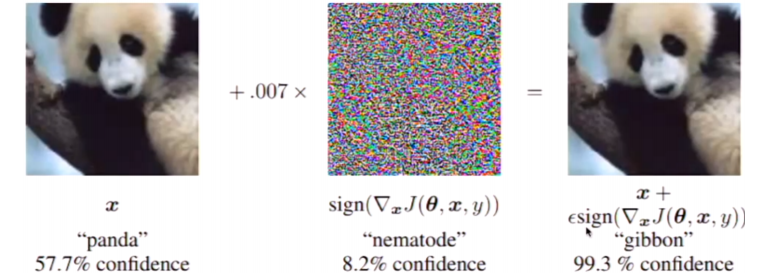
\includegraphics[width=300px, keepaspectratio]{classifiy.png}
    \vspace{1ex}%
    \caption{The output of a variational autoencoder. (Goodfellow, 2015)}
    \label{fig:my_label}
\end{figure}

The structure of a typical VAE model is shown below in Figure 2.10. Image data input is fed into the model. The model begins to encode the image by compressing the data to represent the essential features learned during training. At the bottleneck, which is the red box on the figure, the final encoded data representation of the input is located. This specific image went from four features down to two features. The generative section of the model comes after the bottleneck, where the model attempts to reconstruct the original input image from the encoded input.

\begin{figure}[H]
    \centering
    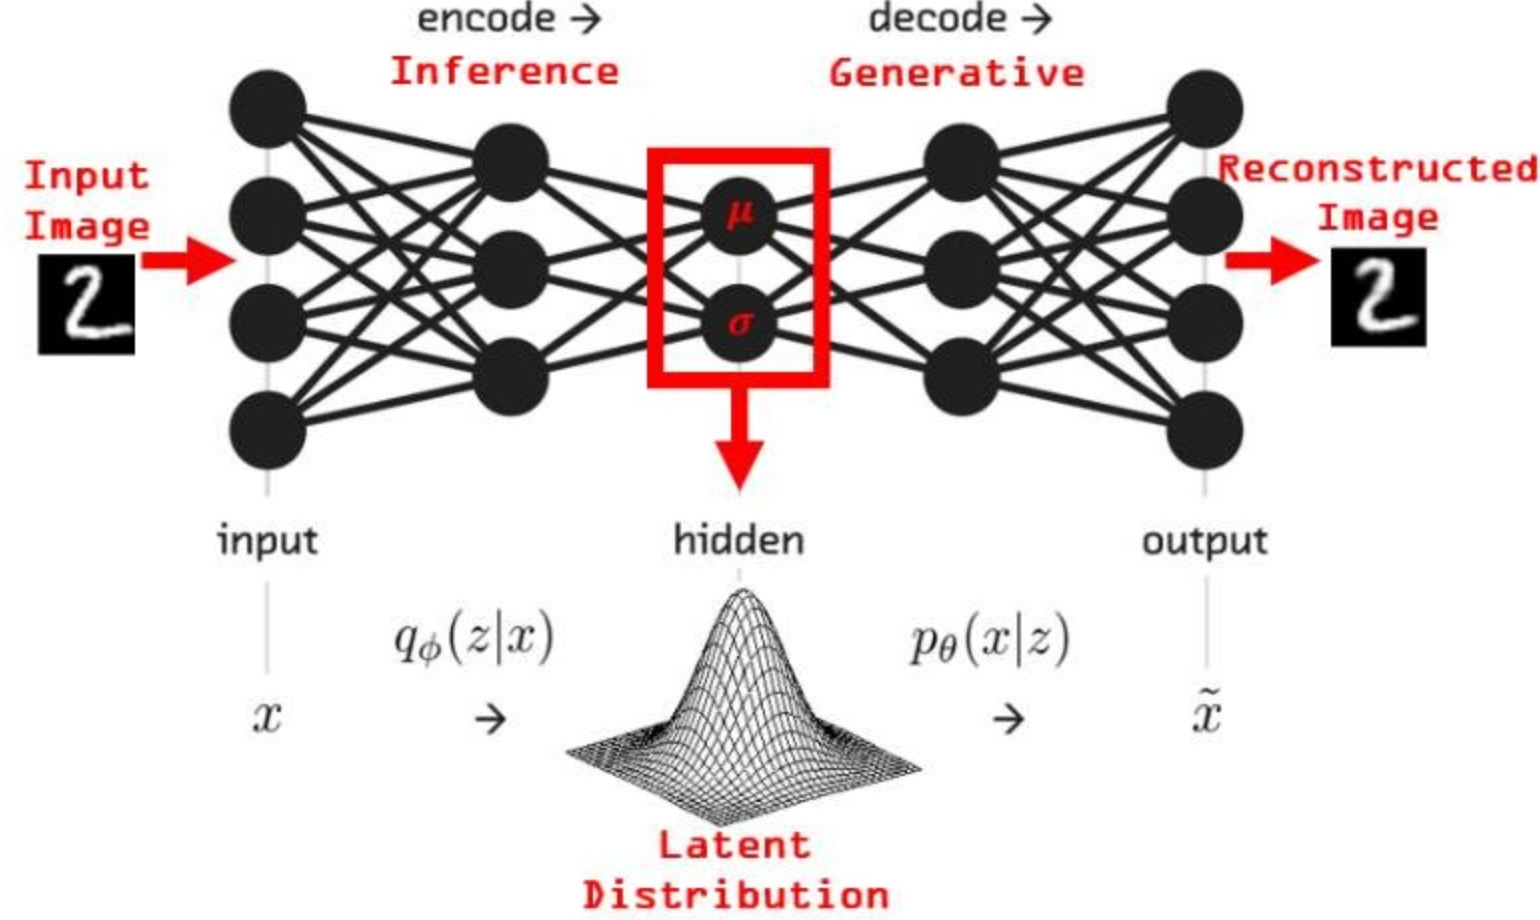
\includegraphics[width=300px, keepaspectratio]{vae.png}
    \vspace{1ex}%
    \caption{The basic structure of a variational autoencoder. (A. Al, 2020)}
    \label{fig:my_label}
\end{figure}
% talk more about other autoencoders for a bit here

Sparse autoencoders (SAE) are a type of autoencoder that follows the general autoencoder structure. However, the critical difference is in how the hidden activations work. SAEs can include equal or more nodes at the bottleneck; however, only a small number of hidden units are allowed to be active simultaneously, creating artificial dynamic bottlenecks. This sparsity constraint forces the model to respond to unique statistical features of the training data, where nodes specialise in categorising particular features. One key advantage of this type of autoencoder is that it has improved performance on classification tasks. Figure 2.11 displays a visual representation of an SAE.

\begin{figure}[H]
    \centering
    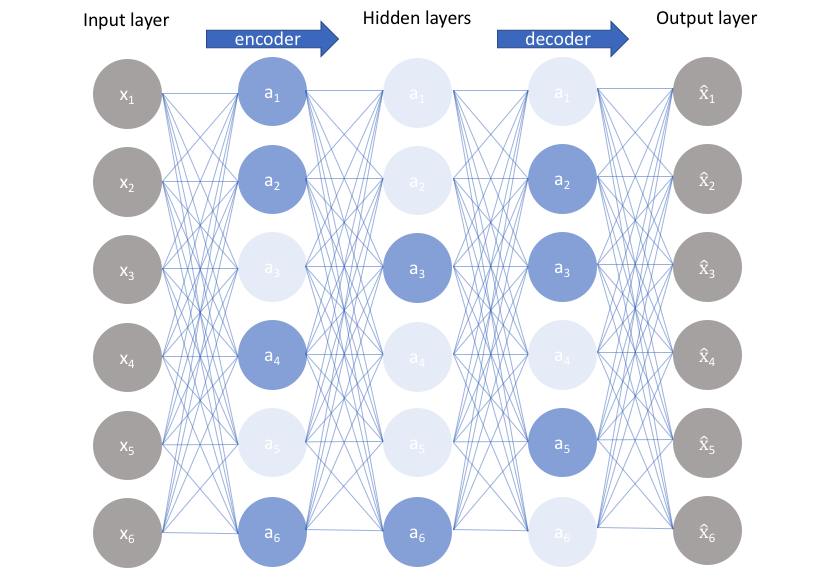
\includegraphics[width=350px, keepaspectratio]{asd.png}
    \vspace{1ex}%
    \caption{Visual representation of a sparse autoencoder, light blue nodes are inactive. (Z. Syoya, 2018)}
    \label{fig:my_label}
\end{figure}


In a study performed by \textit{Jin et al.} [21], VAE networks alongside LSTM networks were used to detect falls using mmWave radar data. The study had first processed mmWave data on ADL to capture doppler features and centroid data for the input frame. This data would then be input fed into a hybrid model that modifies the typical bottleneck of a VAE model. 

Rather than employing a typical bottleneck with hidden layers, a sequence to sequence model is used instead to capture history motion data. The model used is shown in Figure 2.12. 

\begin{figure}[H]
    \centering
    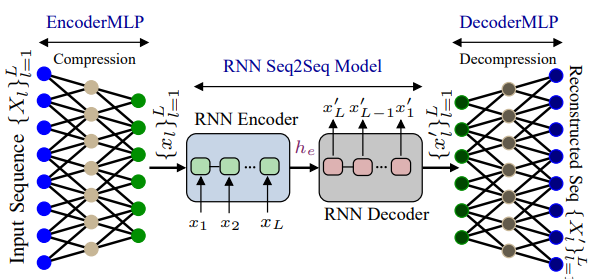
\includegraphics[width=400px, keepaspectratio]{hvae.png}
    \vspace{1ex}%
    \caption{Variational autoencoder with the use of LSTM. (Jin, 2020)}
    \label{fig:my_label}
\end{figure}

The model would output the likelihood of the image reconstruction, and when the model output was below a threshold value, this would indicate an anomaly had occurred. Centroid information is used to investigate anomalies further and reduce false-positive rates. When the centroid height rapidly decreases, alongside detecting an anomaly, this would indicate a fall has occurred. 

To test the model, 50 simulated falls alongside negative samples were created and passed into the model for classification. The result of this study had shown that it had achieved a specificity of 98\% (49/50), and only two false alarms were triggered amongst the negative samples. This method proves extremely promising as it maintains the subjects' privacy while also providing high specificity. However, this method has only been tested on simulated falls, which often cannot represent an actual fall situation. The model has not been tested or designed to work in a real-time environment.  

In another study performed by \textit{Nogas et al.} [24], a deep spatio-convolutional autoencoder (DSCAE) was used to detect falls as anomalies. Video frames stacked together were used as input to the network, where 3D convolutions take place for encoding inputs. Three convolutional layers are used to encode the 8x64x64x1 data into 2x8x8x8 data. Encoded inputs are then up-sampled and sent through further convolutional layers to reconstruct the encoded inputs. Figure 2.13 illustrates a simplified representation of the network structure. 

\begin{figure}[H]
    \centering
    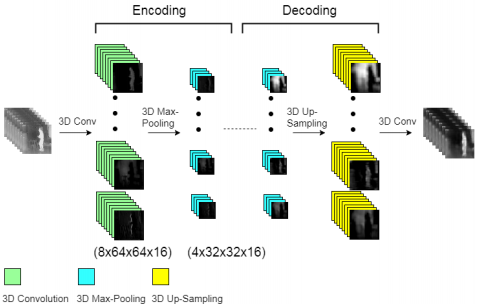
\includegraphics[ keepaspectratio]{eeeeeeee.png}
    \vspace{1ex}%
    \caption{Deep spatio-convolutional autoencoder structure. (Nogas, 2020)}
    \label{fig:my_label}
\end{figure}

The model uses a novel threshold system to determine anomalies. Rather than computing an anomaly score on a frame by frame basis, the model calculates an anomaly score for each frame alongside reconstruction error information in adjacent video frame stacks. This was shown to perform better in real-world scenarios.  

Three different public datasets were used to test the model, thermal fall dataset (TFD), URFD, and the SDU dataset. The result of this study shows that this model outperforms other autoencoder methods and other machine learning approaches. The AUC of the model on the three datasets averaged 0.91, whereas a traditional deep autoencoder approach had an average AUC of 0.78 and a K-nearest neighbour approach had an AUC of 0.58.

\subsection{Data Availability Issues for Fall Detection}
In the field of fall detection using machine learning, acquiring fall data has been a significant challenge. In a study conducted by \textit{Schwickert et al.} [4], it was shown that 94\% of studies use simulated falls for training models, validating models, or both. Fall data is rare, as falls are rare events, and simulating a fall cannot necessarily encapsulate all aspects of a natural fall. 

For supervised learning techniques, this can be problematic for a few reasons. If a model has only been trained to work on simulated falls, it may overfit during training and perform poorly in a real-world event. Falls from healthy young subjects are not the same as a fall from an elderly person [3]. Another issue is that supervised learning methods require a large amount of data for training to ensure the model does not overfit the training dataset; this is especially true in more complex models that must learn more weights. The data provided must also be evenly distributed in output classes to ensure the model is not biased towards a specific output class. Due to the rarity of falls, it would be unrealistic to train a supervised learning model with real fall data due to the lack of real falls. This issue is less problematic for anomaly detection methods as they primarily use ADL data. However, when it comes to testing the models, often simulated falls are used. 

\section{mmWave Data}
Millimeter-wave radar is a new sensing technology that allows for the detection of objects. These radars provide information regarding the range, velocity, and angle of these objects. mmWave is a contactless technology that operates between 30GHz and 300GHZ. The use of small wavelengths allows sub-mm range accuracy and can penetrate through materials such as drywall, plastic, or clothing [25, 26]. Another critical feature of mmWave sensing technology is the ability to preserve user privacy while maintaining motion and positional information. Figure 2.14 shows the processed data from a mmWave radar alongside a camera view. On the left of the image, you can see the person has fallen; however, on the right, we see a point cloud representation of that motion history, abstracting the individual from the motion entirely. 

\begin{figure}[H]
    \centering
    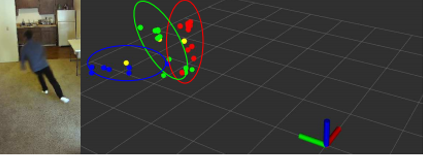
\includegraphics[ keepaspectratio]{asdds.png}
    \vspace{1ex}%
    \caption{Data captured from mmWave sensor visualised. (Jin, 2020)}
    \label{fig:my_label}
\end{figure}

\section{Problem Statement}
Previous studies have shown the difficulty in detecting falls in real-time Often, a study would excel in one aspect of fall detection but present drawbacks that cannot be ignored. Supervised learning models would present a high specificity; however, this is done through simulated falls and often overfit when it comes to real-world scenarios. Supervised learning models also present the privacy concern as often camera feed data is used, placing subjects under constant surveillance. Due to the lack of data available, these models cannot be trained with real fall data. 

Semi-supervised learning approaches seem to do an excellent job in producing models that obtain high specificity and do not require fall data for training. While these models are almost ideal, they continue to use simulated falls to validate the dataset and are not designed to work in real-time. Another issue discovered in the study was that determining a threshold value that minimises false alarms while maximising the correctly classified true positive case was challenging. 

In this thesis, the goal is to create a generative fall detection model that can detect falls as anomalies in real-time while maintaining the subject's privacy and achieving a high specificity on natural falls, with a low rate of false positives. Privacy will be maintained as mmWave radar data will be used (see Figure 2.14). This model will also work 24/7 without placing any responsibility on the subject.

Tensorflow and Keras API will be used to develop the planned model. Edge computers will run locally to collect and process data and pass it onto a pre-trained model to detect falls in real-time.